% Provenance (never printed): see sources/outline_sources.md (Year 3:
% Glen's flow law; mass balance; ice sheets and ice shelves; sea ice;
% permafrost; the cryosphere's contribution to sea level).
% Brief: sources/book5/BRIEFS.md, ch. 24. Curves from figdata/bachelor-3/
% ice_flow.py (Glen slab, the plastic profile against the ETOPO1 Greenland
% transect, the Arkel ice cap) and sea_ice.py (NSIDC March and September
% extents, Stefan's law). Exercise and problem values in the Book 5 scratch
% calculator calc/ch24.py. The Arkel ice cap and the glaciers of the
% exercises are invented.
\chapter{علم الجليد}\label{ch:b3:glaciology}

نعبر غرينلاند من الغرب إلى الشرق على امتداد خط العرض \ang{72.5}شمالًا. يبدأ الجليد
على بعد بضعة عشرات الكيلومترات داخل اليابسة، ثم يرتفع بانحدار شديد، ثم يزداد اعتداله أكثر فأكثر،
حتى قمّة عريضة يبلغ ارتفاعها \qty{3229}{m}، ثم يهبط ثانيةً نحو جبال
الساحل الشرقي. وعند رسمه يقارب السطح قطعًا مكافئًا مستلقيًا على جانبه،
وقمّته عند الحافة. يوضّح هذا الفصل من أين يأتي ذلك الشكل:
من مادّةٍ تزحف أسرع فأسرع كلّما ازداد دفعها،
بحيث تسلك كأنّها لا تتحمّل أكثر من إجهاد معيّن.
ثم يتتبّع الجليد منذ الثلج الذي يغذّيه
حتى البحر الذي يستقبله.
% ledger: data:b5-etopo-greenland

\begin{recall}
النهر الجليدي، والغطاء الجليدي، والرفّ الجليدي، والجبال الجليدية، والجليد البحري، والتربة الصقيعية، وعصور
الجليد مذكورة في كتب المدرسة. وقوانين الانسياب \omterm{def:b3:deformation-mechanisms:creep}{والزحف الانخلاعي} موجودة في
الفصل~\ref{ch:b3:deformation-mechanisms}؛ \omterm{def:b3:gravity-geodesy:satgrav}{وقياس الجاذبية بالأقمار الصناعية}
وميزان كتلة الغطاء الجليدي الذي تقيسه في الفصل~\ref{ch:b3:gravity-geodesy}؛
ولبّات الجليد ونظائر الأكسجين فيها في الفصل~\ref{ch:b3:stable-isotopes}.
وميزانية مستوى سطح البحر، والتغذية الراجعة بين الجليد والألبيدو، وارتفاع
مستوى سطح البحر الحراري موجودة في مجلد السنة الثانية، في فصله عن تغيّر المناخ
البشري المنشأ. وتوجد الحرارة الكامنة والتوصيل الحراري في كتب الفيزياء.
\end{recall}

\section{الجليد كمادّة}\label{sec:b3:glaciology:material}

جليد النهر الجليدي صخرٌ، كتلةٌ من البلورات الجليدية المتشابكة، وهو
يتشوّه قرب نقطة انصهاره. وتحت إجهادٍ يزحف بحركة الانخلاعات
في بلوراته، كما في صخور
الفصل~\ref{ch:b3:deformation-mechanisms}، وقانون انسيابه له الصورة نفسها:
أسٌّ للإجهاد مضروبٌ في عامل أرينيوس.

\begin{theorem}[قانون انسياب غلِن]\label{thm:b3:glaciology:glen}
في جليد النهر الجليدي المتماثل الخواص، يتناسب موتّرُ معدّل الانفعال طرديًّا مع
الإجهاد الانحرافي،
\[
\dot\varepsilon_{ij} = A(T)\,\tau_e^{\,n-1}\,\tau'_{ij}, \qquad
\tau_e^2 = \tfrac12\,\tau'_{ij}\tau'_{ij},
\]
حيث $n = 3$ \omterm{def:b3:glaciology:glen}{وعامل المعدّل} $A(T)$ الذي يتزايد مع درجة الحرارة. وفي
القصّ البسيط، حيث $\tau_{xz}$ هو الإجهاد الانحرافي الوحيد غير المعدوم،
$\dot\varepsilon_{xz} = A\tau_{xz}^{\,n}$.
\end{theorem}
\index{قانون انسياب غلِن}

\begin{proof}
القانون نفسه تجريبيّ: قانونٌ أسّيّ مُطابَقٌ لتجارب الزحف
ولتشوّه الأنهار الجليدية، ومعامله وأسّه مُطابَقان
معًا. وفي القصّ البسيط $\tau'_{xz} = \tau'_{zx} = \tau_{xz}$ وتكون
بقيّة المركّبات معدومةٌ، ومنه $\tau_e^2 = \tfrac12(\tau_{xz}^2 +
\tau_{zx}^2) = \tau_{xz}^2$، و$\dot\varepsilon_{xz} = A\tau_{xz}^{\,n-1}
\tau_{xz}$.
\end{proof}
% ledger: pism:rheology

مع $n = 3$، يكون الجليد مائعًا شديد اللاخطية: مضاعفة الإجهاد تجعله
يتشوّه أسرع ثماني مرّات. واللزوجة الفعّالة $1/(2A\tau_e^{\,2})$،
ليست خاصيّةً للجليد وحده، بل تتناقص مع ارتفاع الإجهاد.

\begin{definition}[عامل المعدّل (الجليد)]\label{def:b3:glaciology:glen}
\emph{عامل المعدّل}\index{عامل المعدّل (الجليد)} $A(T)$ لقانون غلِن، ويُسمّى أيضًا
ليونةَ الجليد، ويُكتب $A = A_0\exp(-Q/RT)$، مع
طاقةَ تنشيط $Q$. وتأخذ ملاءمةٌ شائعةُ الاستعمال (باترسون وبَد) $A_0 =
\qty{3.61e-13}{s^{-1}.Pa^{-3}}$ و$Q = \qty{60}{kJ/mol}$ تحت
\qty{-10}{\celsius}، و$A_0 = \qty{1.73e3}{s^{-1}.Pa^{-3}}$ و$Q =
\qty{139}{kJ/mol}$ فوقها، وأقرب إلى نقطة الانصهار، حيث يلين
الجليد أسرع مع درجة الحرارة.
\end{definition}
% ledger: pism:rheology, codata:R

\begin{center}
\begin{tabular}{lccc}
\hline
درجة الحرارة & \qty{-25}{\celsius} & \qty{-10}{\celsius} & \qty{0}{\celsius}\\
\mbox{\textdir TLT $A$ (\unit{Pa^{-3}.yr^{-1}})} & \num{2.7e-18} & \num{1.4e-17} & \num{1.4e-16}\\
\hline
\end{tabular}
\end{center}

يتدفّق الجليد عند نقطة انصهاره نحو خمسين مرّة أسرع من
\qty{-25}{\celsius} تحت الإجهاد نفسه. والإجهادات في الأنهار الجليدية من
رتبة البار، \qty{e5}{Pa}.
% ledger: pism:rheology

يتحرّك النهر الجليدي بطريقتين. يتشوّه جليده بالزحف في كلّ مكان؛ وحيث
يكون القاع عند نقطة الانصهار، فقد ينزلق أيضًا.

\begin{definition}[الانزلاق القاعدي]\label{def:b3:glaciology:sliding}
\emph{الانزلاق القاعدي}\index{الانزلاق القاعدي} هو حركة النهر الجليدي فوق
قاعه، على غشاء رقيق من الماء أو طبقة من رواسب طرية رطبة. ويقتضي
قاعًا عند نقطة الانصهار؛ والنهر الجليدي المتجمّد بقاعه لا يتحرّك
إلّا بزحف جليده.
\end{definition}
% ledger: nsidc:glacier-flow

\section{انسياب النهر الجليدي}\label{sec:b3:glaciology:flow}

\begin{theorem}[انسياب لوح متوازي الجانبين]\label{thm:b3:glaciology:slab}
يستقرّ لوحٌ من الجليد سمكُه $H$ وكثافتُه $\rho$ على قاعٍ ميله
$\alpha$، ويجري على طوله بالقصّ البسيط، منزلقًا بسرعة $u_b$. وعند
ارتفاع $z$ فوق القاع يكون إجهاد القصّ $\tau = \rho g(H - z)\sin\alpha$،
والسرعة
\[
u(z) = u_b + \frac{2A}{n + 1}(\rho g\sin\alpha)^n\left[H^{n+1} - (H -
z)^{n+1}\right],
\]
والدفق لكلّ وحدة عرض $q = u_bH + \dfrac{2A}{n + 2}(\rho
g\sin\alpha)^nH^{n+2}$. وإجهاد القصّ القاعدي هو $\tau_b = \rho gH\sin\alpha$.
\end{theorem}

\begin{proof}
الجليدُ الواقع فوق الارتفاع $z$ وزنُه $\rho g(H - z)$ لكلّ وحدة مساحة؛ ومركّبتُه
على طول المنحدر، $\rho g(H - z)\sin\alpha$، يوازنها إجهادُ القصّ عند قاعدته، والسطحُ خالٍ من الإجهاد.
بحسب قانون غلِن،
$\mathrm du/\mathrm dz = 2\dot\varepsilon_{xz} = 2A\tau^n$؛ وبالتكامل انطلاقًا
من القاع، حيث $u = u_b$، نحصل على $u(z)$، وبتكامل $u$ من 0 إلى $H$
نحصل على $q$.
\end{proof}

تتغيّر السرعة قليلًا في الجزء العلوي من اللوح، وتتغيّر بسرعة قرب
القاع، حيث يبلغ الإجهاد أقصاه: مع $n = 3$ يتركّز القصّ في
أدنى الطبقات. وتتناسب السرعة السطحية مع $H^{n+1} = H^4$ ومع مكعّب
الميل: فالنهر الجليدي الذي سماكتُه ضعفُ غيره يجري أسرعَ منه ستّ عشرة مرّة.

\begin{definition}[تقريب الجليد الضحل]\label{def:b3:glaciology:sia}
يعامل \emph{تقريب الجليد الضحل}\index{تقريب الجليد الضحل} غطاءً جليديًّا
تكون سماكتُه صغيرةً قياسًا إلى عرضه، بوصفه محليًّا
لوحًا متوازيَ الجانبين: عند كلّ موضع يتشوّه الجليد بالقصّ البسيط تحت
\emph{إجهاد الدفع} $\tau_d = \rho gH|\nabla s|$، حيث $s$
الارتفاعُ السطحي، ويتبع الدفقُ صيغةَ اللوح بالسماكة المحليّة
والميل السطحي.
\end{definition}

في \omterm{def:b3:glaciology:sia}{تقريب الجليد الضحل} يتحدّد الإجهادُ القاعدي بشكل
الجليد. ولأنّ معدّل الانفعال يتناسب مع مكعّب الإجهاد، تؤدّي زيادةٌ معتدلةٌ
في الإجهاد إلى زيادة كبيرة في الجريان، فيُرقّق الجليد
ويُخفّض الإجهادَ من جديد: يبقى الإجهاد ضمن مدًى ضيّق،
أيًّا كان حجمُ الكتلة الجليدية. ولنأخذ ذلك إلى حدّه الأقصى: مادّةٌ
لا تتشوّه البتّةَ دون إجهاد خضوع $\tau_0$، وتتشوّه بلا حدّ
فوقه، ويتبع الشكلُ ذلك.

\begin{proposition}[مقطع الغطاء الجليدي اللدن]\label{prop:b3:glaciology:nye}
غطاءٌ جليدي لدن تمامًا، إجهاد خضوعه $\tau_0$، على قاعٍ أفقيّ مستوٍ
يكون له، على المسافة $x$ داخل اليابسة من حافّته، ارتفاعُ السطح
\[
h(x) = \sqrt{\frac{2\tau_0x}{\rho g}} .
\]
\end{proposition}
\index{مقطع الغطاء الجليدي اللدن}

\begin{proof}
في كلّ موضع يساوي الإجهاد القاعدي إجهاد الخضوع: $\rho gh\,\mathrm
dh/\mathrm dx = \tau_0$، إذ الميلُ صغيرٌ. ثمّ $\mathrm d(h^2)/\mathrm
dx = 2\tau_0/(\rho g)$، و$h = 0$ عند الحافّة.
\end{proof}

\begin{omfigure}
\begin{tikzpicture}
\begin{groupplot}[group style={group size=2 by 1, horizontal sep=1.5cm},
  height=0.4\linewidth,
  tick label style={font=\scriptsize}, label style={font=\small}, title style={font=\small}]
\nextgroupplot[width=0.38\linewidth, xlabel={$u/u_s$}, ylabel={الارتفاع فوق القاع، $z/H$},
  xmin=0, xmax=1.05, ymin=0, ymax=1, title={لوح جليدي},
  legend style={font=\scriptsize, at={(0.03,0.97)}, anchor=north west}]
% computed in figdata/bachelor-3/ice_flow.py
\addplot[omThm, thick] table[x=u3, y=zeta] {figdata/out/bachelor-3-ice_flow-slab.dat};
\addlegendentry{$n = 3$}
\addplot[omDef, thick, densely dashed] table[x=u1, y=zeta] {figdata/out/bachelor-3-ice_flow-slab.dat};
\addlegendentry{$n = 1$}
\addplot[omMeth, thick] table[x=u3b, y=zeta] {figdata/out/bachelor-3-ice_flow-slab.dat};
\addlegendentry{\foreignlanguage{arabic}{\mbox{\textdir TLT $n = 3$}، الانزلاق القاعدي}}
\nextgroupplot[width=0.58\linewidth, xlabel={المسافة من \ang{58}غربًا على طول \ang{72.5}شمالًا \babelsublr{(\unit{km})}},
  ylabel={الارتفاع \babelsublr{(\unit{m})}}, xmin=0, xmax=1270, ymin=-500, ymax=3700,
  title={غرينلاند}, scaled x ticks=false, xticklabel style={/pgf/number format/1000 sep={}},
  scaled y ticks=false, yticklabel style={/pgf/number format/1000 sep={}},
  legend style={font=\scriptsize, at={(0.5,0.03)}, anchor=south}]
\addplot[black, thin] table[x=x, y=h] {figdata/out/bachelor-3-ice_flow-gl.dat};
\addlegendentry{الجليد وسطح اليابسة}
\addplot[omThm, thick, densely dashed] table[x=x, y=h] {figdata/out/bachelor-3-ice_flow-nye-w.dat};
\addlegendentry{المقاطع اللدنة}
\addplot[omThm, thick, densely dashed, forget plot] table[x=x, y=h] {figdata/out/bachelor-3-ice_flow-nye-e.dat};
\draw[black!40] (axis cs:0,0) -- (axis cs:1270,0);
\node[font=\scriptsize, omThm, align=center] at (axis cs:330,2900) {$\tau_0 = $\\ \qty{72}{kPa}};
\node[font=\scriptsize, omThm, align=center] at (axis cs:1040,2900) {$\tau_0 = $\\ \qty{108}{kPa}};
\end{groupplot}
\end{tikzpicture}

\par\smallskip{\small يسارًا، السرعة عبر لوح جليدي، مُقاسةً بسرعة
السطح: قانونُ غلِن ($n = 3$) يركّز القصّ قرب القاع، أمّا
المائعُ الخطّي ($n = 1$) فيوزّعه؛ ومع \omterm{def:b3:glaciology:sliding}{الانزلاق القاعدي} يكون المقطعُ كلّه
مُزاحًا. يمينًا، سطح غرينلاند على امتداد \ang{72.5}شمالًا \babelsublr{(ETOPO1 Ice Surface, NOAA NCEI)}،
والمقاطعُ اللدنةُ المُلائَمةُ لجانبيه، للارتفاعات
فوق \qty{1000}{m}، والقاعُ مأخوذٌ عند مستوى سطح البحر. وتتطلّب الملاءمةُ
إجهادَيْ خضوعٍ \qty{72}{kPa} و\qty{108}{kPa}، وهما من رتبة البار لدى
الأنهار الجليدية الحقيقية؛ ولا تُطابق الحافّاتِ الشديدةَ الانحدار، حيث يكتسب القاع والانصهار
أهميةً حاسمة.}\label{fig:b3:glaciology:flow}
\end{omfigure}
% ledger: data:b5-etopo-greenland, pism:rheology

\section{ميزان الكتلة}\label{sec:b3:glaciology:mass-balance}

يتغذّى النهر الجليدي بالثلج، ويفقد الجليدُ بالانصهار والتبخّر، وحيثما
يبلغ الماءَ، \omterm{def:b3:glaciology:grounding-line}{بانفصال الجبال الجليدية}.
% ledger: nsidc:glacier-zones

\begin{definition}[ميزان الكتلة؛ نطاقا التراكم والاستنزاف؛ خط التوازن]\label{def:b3:glaciology:mass-balance}
\emph{ميزان كتلة النهر الجليدي}\index{ميزان كتلة النهر الجليدي} هو التغيّر في كتلة
النهر الجليدي خلال سنة، ويُعطى عادةً بالأمتار من الماء
المكافئ متوسّطًا على مساحته. و\emph{ميزان الكتلة السطحي}\index{ميزان الكتلة السطحي} هو
الجزءُ منه الناتج عن العمليات الجارية عند السطح، أي تساقط الثلج ناقصًا الانصهار،
والجريانَ السطحي والتسامي؛ أمّا الباقي فيُفقَد
\omterm{def:b3:glaciology:grounding-line}{بانفصال الجبال الجليدية} وبالانصهار عند القاعدة أو تحت الجليد العائم. ويُسمّى
\emph{نطاق التراكم}\index{نطاق التراكم} الجزءَ من السطح الذي يكون فيه ميزانُ الكتلة السطحي
خلال سنة موجبًا،
و\emph{نطاق الاستنزاف}\index{نطاق الاستنزاف} الجزءَ الذي يكون فيه سالبًا،
و\emph{ارتفاع خط التوازن}\index{ارتفاع خط التوازن}
\babelsublr{(ELA)} هو ارتفاع الخطّ الفاصل بينهما، حيث يكون الميزان معدومًا.
\end{definition}

\begin{omfigure}
\centering
\begin{tikzpicture}[>=stealth, font=\small, x=1cm, y=1cm]
% bed and surface of a valley glacier, long section
\fill[black!12] (0,0) -- (0,4.6) .. controls (2,3.6) and (6,1.4) .. (11,0) -- cycle;
\fill[omSea!45] (0,4.6) .. controls (2,3.6) and (6,1.4) .. (11,0)
  -- (11,0) .. controls (8,1.0) and (4,3.2) .. (0.6,5.4) -- (0,5.6) -- cycle;
\draw[thick, black!70] (0,4.6) .. controls (2,3.6) and (6,1.4) .. (11,0);
\draw[thick, omDef] (0,5.6) -- (0.6,5.4) .. controls (4,3.2) and (8,1.0) .. (11,0);
% equilibrium line
\draw[omThm, densely dashed, thick] (5.0,2.76) -- (5.0,4.6);
\node[omThm, font=\scriptsize, anchor=south] at (5.0,4.6) {\foreignlanguage{arabic}{خط التوازن \mbox{\textdir TLT (ELA)}}};
% balance arrows
\foreach \x/\y in {1.2/5.02, 2.4/4.27, 3.6/3.56} {\draw[->, omDef, thick] (\x,\y+0.55) -- (\x,\y+0.05);}
\foreach \x/\y in {6.4/2.02, 7.6/1.42, 8.8/0.86} {\draw[->, omThm, thick] (\x,\y+0.02) -- (\x,\y+0.52);}
\node[omDef, font=\scriptsize, align=center] at (2.4,6.2) {\foreignlanguage{arabic}{نطاق التراكم:}\\الثلج المكتسب};
\node[omThm, font=\scriptsize, align=center] at (8.6,2.5) {\foreignlanguage{arabic}{نطاق الاستنزاف:}\\الجليد المفقود};
% flow lines, computed inside the ice: buried in the accumulation zone, emerging in the ablation zone
\draw[->, black!60] plot[smooth] coordinates {(1.00,5.14) (1.98,4.28) (2.95,3.54) (3.93,2.93) (4.90,2.43) (5.88,2.00) (6.85,1.62) (7.83,1.24) (8.80,0.86)};
\draw[->, black!60] plot[smooth] coordinates {(2.20,4.39) (2.84,3.89) (3.48,3.43) (4.11,3.02) (4.75,2.67) (5.39,2.36) (6.03,2.08) (6.66,1.82) (7.30,1.56)};
\draw[->, black!60] plot[smooth] coordinates {(3.40,3.67) (3.74,3.44) (4.08,3.21) (4.41,3.00) (4.75,2.81) (5.09,2.63) (5.42,2.47) (5.76,2.32) (6.10,2.17)};
\node[font=\scriptsize, anchor=north east] at (10.9,-0.1) {الجبهة};
\node[font=\scriptsize] at (3.0,1.4) {الصخر الأساسي};
\end{tikzpicture}

\par\smallskip{\small مقطع طولي تخطيطي لنهر جليدي واديّ في
حالة توازن. فوق خط التوازن يُدفن ثلج كلّ سنة ويُنقل إلى
داخل النهر الجليدي؛ أما تحت الخط فيفقد السطح جليدًا كلّ سنة
ويُعوَّض بجليد صاعد من الأعماق. تنحدر خطوط الجريان (الرمادية) في \omterm{def:b3:glaciology:mass-balance}{نطاق التراكم}
وترتفع في \omterm{def:b3:glaciology:mass-balance}{نطاق الاستنزاف}؛ ويحمل الجريان
فائض \omterm{def:b3:glaciology:mass-balance}{نطاق التراكم} إلى عجز \omterm{def:b3:glaciology:mass-balance}{نطاق الاستنزاف}.}\label{fig:b3:glaciology:zones}
\end{omfigure}
% ledger: nsidc:glacier-zones, nsidc:glacier-flow

على الأغطية الجليدية والأنهار الجليدية المرتفعة، لا يتحوّل الثلج إلى جليد
خلال فصل واحد. يُدفن بثلج لاحق، ويُضغط، ويُعاد تبلوره.

\begin{definition}[الفِرن؛ انغلاق المسام]\label{def:b3:glaciology:firn}
\emph{الفِرن}\index{الفِرن} ثلج نجا من موسم انصهار واحد على الأقل
ويجري ضغطه ليتحوّل إلى جليد: أكثف من الثلج، ولا يزال نفّاذًا للهواء.
\emph{انغلاق المسام}\index{انغلاق المسام} هو النقطة في
عملية ضغطه، عند كثافة تقارب \qtyrange{820}{830}{kg/m^3}، حيث
تُغلق المسام بين الحبيبات وتتحوّل إلى فقاعات، ويُعزل الهواء الذي فيها
عن الغلاف الجوي.
\end{definition}

في الأغطية الجليدية القطبية يقع \omterm{def:b3:glaciology:firn}{انغلاق المسام} على عمق \qtyrange{50}{120}{m} تحت
السطح، ويتوقّف ذلك على درجة الحرارة والتراكم
والشوائب؛ ولذلك يكون الهواء في فقاعات لبّ الجليد أحدث من
الجليد المحيط به، كما ذكر الفصل~\ref{ch:b3:stable-isotopes}. وبالنسبة إلى معظم
الأنهار الجليدية يستغرق التحوّل من الثلج إلى الجليد أكثر من مئة سنة.
% ledger: nsidc:firn, firn:close-off

لا يستجيب النهر الجليدي فورًا لتغيّر مناخه. يجب أن يتغيّر سُمكه
قبل أن يستطيع طوله أن يتبعه.

\begin{proposition}[زمن استجابة النهر الجليدي]\label{prop:b3:glaciology:response}
نهرٌ جليدي سُمكه المميّز $H$ وميزانه عند طرفه $b_t <
0$ (بالأمتار من الجليد في السنة) يتكيّف مع تغيّر المناخ خلال زمن
من رتبة
\[
\tau = \frac{H}{-b_t} .
\]
\end{proposition}

\begin{proof}
يغيّر تغيّرُ الميزان بمقدار $\delta b$ على النهر الجليدي حجمَه
إلى أن تُعوَّض المساحة المفقودة أو المكتسبة عند الطرف، حيث الميزان $b_t$،
تُعوِّضه: $L\,\delta b = -b_t\,\delta L$ لكل وحدة عرض، من أجل نهر
جليدي طوله $L$. يبلغ تغيّر الحجم اللازم نحو $H\,\delta L$،
وإنّ الاختلال الذي يدفعه هو $L\,\delta b$ في السنة، في البداية، فيستغرق
التغيّر $H\,\delta L/(L\,\delta b) = H/(-b_t)$ سنة.
\end{proof}

نهرٌ جليدي سُمكه \qty{200}{m} يفقد \qty{5}{m} من الجليد كلّ سنة عند
لسانه يحتاج إلى نحو أربعين سنة لكي يستجيب. لذلك تتأخر الأنهار الجليدية عن
المناخ: فالأنهار الجليدية اليوم ستواصل فقدان كتلتها لعقود حتى لو
توقّفت درجة الحرارة عن الارتفاع.
% ledger: ar6ch9:glaciers

\section{الأغطية الجليدية والرفوف الجليدية}\label{sec:b3:glaciology:ice-sheets}

تحتوي الأغطية الجليدية في غرينلاند والقارة القطبية الجنوبية على أكثر من
\qty{99}{\percent} من الجليد البرّي. يبلغ غطاء غرينلاند \qty{1.7}{\mega
km^2} وسُمكه يتجاوز \qty{3}{km} على الأكثر؛ أما غطاء القارة القطبية الجنوبية فيبلغ
قرابة \qty{14}{\mega km^2} وسُمكه يقارب \qty{4.9}{km} على الأكثر. وتستقرّ أجزاء كثيرة
من الغطاء الجليدي القطبي الجنوبي على قاع يقع تحت مستوى سطح البحر.
% ledger: nsidc:ice-sheets, ar6ch9:faq91

\begin{definition}[التيار الجليدي]\label{def:b3:glaciology:ice-stream}
\emph{التيار الجليدي}\index{التيار الجليدي} هو نطاق من غطاء جليدي يجري
أسرع بكثير من الجليد على جانبيه، وذلك في الغالب بالانزلاق أو بتشوّه
قاعٍ طريٍّ رطب، ويُصرِّف جزءًا كبيرًا من داخل الغطاء الجليدي
نحو حافّته.
\end{definition}

\begin{definition}[خط الارتكاز؛ انفصال الجبال الجليدية]\label{def:b3:glaciology:grounding-line}
\emph{خط الارتكاز}\index{خط الارتكاز} هو الخط الذي يبدأ عنده الجليد
المستقرّ على قاعه بالطفو: وعلى الجهة البحرية منه يكون الجليد رفًّا جليديًّا
أو لسانًا جليديًا عائمًا. \emph{انفصال الجبال الجليدية}\index{انفصال الجبال الجليدية} هو تكسّر
كُتل من الجليد، أي الجبال الجليدية، عند جبهة النهر الجليدي أو الرفّ الجليدي
الذي ينتهي في الماء.
\end{definition}

تطفو الرفوف الجليدية، ولذلك لا يرفع انصهارها مستوى سطح البحر. لكنّها
مُثبَّتة من جانبيها وعلى مرتفعات قاع البحر حيث تجنح
على القاع، ويقاوم الاحتكاك هناك جريان الجليد خلفها: فهي
\emph{تُسنده}. بعد تفكّك الرفّ الجليدي لارسن~B في عام 2002، تسارعت
الأنهار الجليدية التي كانت تغذّيه، حتى ثماني مرات.
% ledger: nsidc:ice-shelves

\begin{proposition}[الطفو]\label{prop:b3:glaciology:flotation}
جليد كثافته $\rho_i$ وسُمكه $H$ فوق قاع على عمق $D$ تحت مستوى سطح البحر،
في ماء بحر كثافته $\rho_w$، يطفو إذا كان $H < (\rho_w/\rho_i)D$.
مع $\rho_i = \qty{917}{kg/m^3}$ و$\rho_w = \qty{1025}{kg/m^3}$، يقع
\omterm{def:b3:glaciology:grounding-line}{خط الارتكاز} حيث يكون الجليد سُمكه $1.12\,D$.
\end{proposition}

\begin{proof}
يُزيح الجليد العائم وزنًا من الماء مساويًا لوزنه: عمودٌ سُمكه $H$
يحتاج إلى غاطس $\rho_iH/\rho_w$. فإذا كان الماء أعمق من هذا الغاطس،
فإنّ الجليد يطفو.
\end{proof}
% ledger: iapws:ice-density, noaa:seawater-1025

\begin{omfigure}
\centering
\begin{tikzpicture}[>=stealth, font=\small, x=1cm, y=1cm]
% sea and bed
\fill[omSea!50] (4.2,0) rectangle (11,-2.8);
\fill[black!15] (0,-0.9) -- (2.2,-2.0) -- (4.6,-1.6) -- (7.0,-2.3) -- (11,-2.6)
  -- (11,-3.2) -- (0,-3.2) -- cycle;
\draw[thick, black!60] (0,-0.9) -- (2.2,-2.0) -- (4.6,-1.6) -- (7.0,-2.3) -- (11,-2.6);
% grounded ice and ice shelf
\fill[white] (0,-0.9) -- (0,2.4) .. controls (2,2.2) and (3.6,1.4) .. (4.6,0.2)
  -- (9.2,0.12) -- (9.2,-1.0) -- (4.6,-1.6) -- (2.2,-2.0) -- cycle;
\draw[thick, omDef] (0,2.4) .. controls (2,2.2) and (3.6,1.4) .. (4.6,0.2) -- (9.2,0.12)
  -- (9.2,-1.0) -- (4.6,-1.6);
\draw[thick] (0,0) -- (0,0);
\draw[omDef!60, thin] (0,0) -- (4.3,0); \draw[omDef!60, thin] (9.2,0) -- (11,0);
\node[font=\scriptsize, anchor=south west] at (0.05,0.02) {مستوى سطح البحر};
% icebergs
\fill[white] (10.1,0.1) rectangle (10.6,-0.7); \draw[omDef] (10.1,0.1) rectangle (10.6,-0.7);
% labels
\fill[omThm] (4.6,-1.6) circle (0.07);
\draw[omThm, ->] (4.0,-2.6) node[anchor=north, font=\scriptsize] {خط الارتكاز} -- (4.55,-1.68);
\node[font=\scriptsize] at (1.4,1.1) {الغطاء الجليدي المرتكز};
\node[font=\scriptsize] at (6.9,-0.7) {الرفّ الجليدي العائم};
\node[font=\scriptsize, anchor=south] at (9.2,0.2) {جبهة الانفصال};
\node[font=\scriptsize, anchor=north, align=center] at (10.35,-0.8) {جبل جليدي};
\node[font=\scriptsize, align=center] at (2.1,-2.55) {القاع يتعمّق\\نحو الداخل};
\draw[->, black!60, thick] (2.2,1.6) -- (3.6,1.0);
\draw[->, black!60, thick] (5.4,-0.2) -- (7.0,-0.2);
\node[font=\scriptsize, align=center, omMeth] at (7.0,1.2) {الإسناد: احتكاك عند جانبي الرفّ\\وعند المرتفعات المرتكزة};
\draw[->, omMeth, thick] (7.6,0.6) -- (6.6,0.6);
\end{tikzpicture}

\par\smallskip{\small مقطع تخطيطي لغطاء جليدي بحري، غير مرسوم
بمقياس. يرتكز الجليد على قاع دون مستوى سطح البحر يتعمّق نحو الداخل؛ وعند
\omterm{def:b3:glaciology:grounding-line}{خط الارتكاز} يبدأ بالطفو بوصفه رفًّا جليديًّا، فيفقد الجليد
بالانفصال عند جبهته وبالانصهار من الأسفل. ويقاوم الاحتكاك في الرفّ حيث
يُسنَد من جانبيه وعلى مرتفعات قاع البحر، فيقاوم انسياب
الجليد المرتكز.}\label{fig:b3:glaciology:grounding}
\end{omfigure}
% ledger: nsidc:ice-shelves, ar6ch9:misi

على قاع يتعمّق نحو الداخل يكون \omterm{def:b3:glaciology:grounding-line}{خط الارتكاز} هشًّا. وحيث
الماء أعمق يكون الجليد عند \omterm{def:b3:glaciology:grounding-line}{خط الارتكاز} أسمك، بحسب شرط الطفو،
وبحسب مبرهنة الشريحة يتزايد دفق العمود الأسمك
بشدّة مع سمكه. فإذا تراجع \omterm{def:b3:glaciology:grounding-line}{خط الارتكاز} على مثل هذا
المنحدر، وصل إلى جليد أسمك يُصرِّف كمية أكبر، ويصبح أرقّ بسرعة أكبر، فيسمح
ذلك للخط بالتراجع أكثر.

\begin{definition}[عدم استقرار الغطاء الجليدي البحري]\label{def:b3:glaciology:misi}
\emph{عدم استقرار الغطاء الجليدي البحري}\index{عدم استقرار الغطاء الجليدي البحري}
\babelsublr{(MISI)} هو التراجع المقترَح ذاتيّ التعزيز \omterm{def:b3:glaciology:grounding-line}{لخط الارتكاز} لغطاء جليدي
يرتكز على قاع ينحدر نحو الداخل: من دون
الإسناد الذي يوفّره رفّ جليدي، يكون \omterm{def:b3:glaciology:grounding-line}{خط الارتكاز} على هذا القاع
غير مستقرّ بطبيعته إلى أن يصل إلى قاع ينحدر نحو الأعلى.
\end{definition}

يمكن لرفوف الجليد أن تُبقي \omterm{def:b3:glaciology:grounding-line}{خط الارتكاز} في مكانه حتى على منحدر نحو الأسفل.
تُظهر النماذج التي تُزال فيها جميع رفوف الجليد في أنتاركتيكا ولا يُسمح لها
بإعادة تكوّنها، تفقد جليدًا يعادل \qtyrange{2}{10}{m} من مستوى سطح البحر خلال 500
عامًا بسبب عدم الاستقرار هذا، منها \qtyrange{2}{5}{m} من غرب
أنتاركتيكا. وفي الغطاء الجليدي المرتكز في معظمه على صخر أساسي فوق مستوى سطح البحر، مثل
غرينلاند، فالعملية الرئيسية ذاتيّة التعزيز مختلفة: فحين يذوب السطح ويهبط،
يصبح في هواء أدفأ فيذوب أكثر.
% ledger: ar6ch9:misi, ar6ch9:faq91

\begin{definition}[مكافئ مستوى سطح البحر]\label{def:b3:glaciology:sle}
\emph{مكافئ مستوى سطح البحر}\index{مكافئ مستوى سطح البحر} لكتلة من
الجليد البرّي هو الارتفاع في متوسط مستوى سطح البحر العالمي الذي كان سيُحدثه ذوبانها
لو انتشر الماء فوق المحيط الحالي.
\end{definition}

\begin{proposition}[مكافئ مستوى سطح البحر لكتلة من الجليد]\label{prop:b3:glaciology:sle}
كتلة $M$ من الجليد المرتكزة فوق مستوى سطح البحر، موزّعةً على محيط مساحته
$A_o$ على هيئة ماء كثافته $\rho_w$، فترفع مستوى سطح البحر بمقدار $M/(\rho_wA_o)$:
نحو \qty{1}{mm} لكل \qty{360}{Gt}.
\end{proposition}

\begin{proof}
يشغل الماء الحجم $M/\rho_w$ على المساحة $A_o$. وباعتماد
\qty{360}{Gt} لكل مليمتر الذي تعتمده تقديرات ميزان كتلة الغطاء الجليدي،
فيكون $A_o\rho_w = \qty{3.6e17}{kg/m}$: محيطًا مساحته نحو
\qty{3.6e8}{km^2} لماء بكثافة الماء العذب.
\end{proof}
% ledger: data:b5-imbie

الجليد الواقع أصلًا تحت مستوى سطح البحر يزيح ماء البحر، فيُحسب بقيمة أقلّ:
جليد القارة القطبية الجنوبية البالغ \qty{30}{\mega km^3} يعادل نحو
\qty{58}{m} من مستوى سطح البحر، وهو أقلّ من كتلته مقسومةً على
\qty{360}{Gt/mm}.
% ledger: nsidc:ice-sheets

\begin{omfigure}
\centering
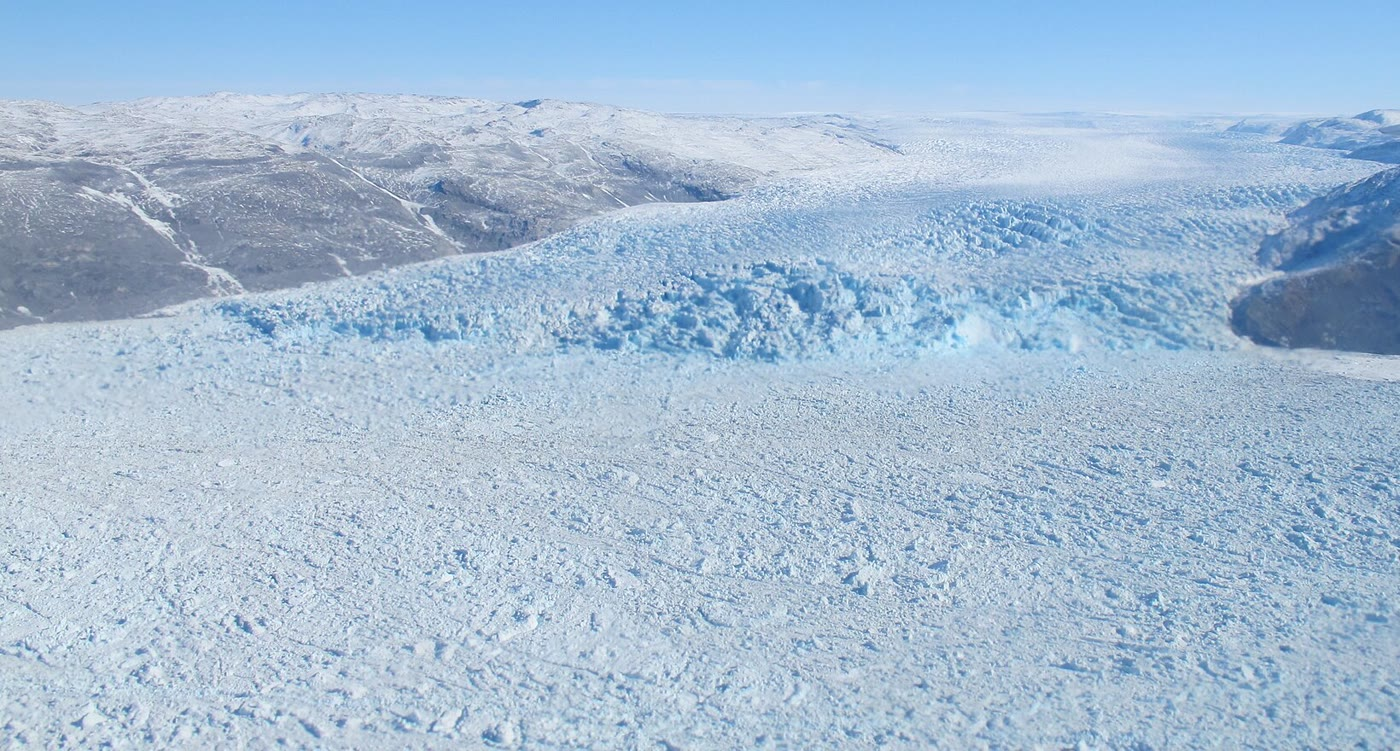
\includegraphics[width=0.82\linewidth]{images/book5/b3-greenland-outlet.jpg}

\par\smallskip{\small نهر جليدي مُصرِّف من الغطاء الجليدي في غرينلاند،
يقع بين الجبال وينتهي في البحر عند جبهة الانفصال، وهو الجدار المكسور
من الجليد الأزرق عبر وسط الصورة؛ والفيورد أمامه مسدود
بالجليد المنفصل وجليد البحر. صُوِّرت من طائرة تابعة لوكالة NASA
في عملية \babelsublr{Operation IceBridge} في أبريل 2014 (الصورة: \mbox{\textdir TLT NASA / Jim Yungel}، ملك
عام).}\label{fig:b3:glaciology:outlet}
\end{omfigure}
% ledger: photo:b3-greenland-outlet

\begin{inthefield}[مخيّم على الجليد]
\begin{minipage}[t]{0.55\linewidth}\vspace{0pt}
على الغطاء الجليدي تنتقل أجهزة علماء الجليد بالزلّاجات وتقيم في
الخيام. ولقياس سرعة حركة الجليد يُثبّتون عمودًا في
الثلج ويثبّتون عليه هوائي مستقبِل للملاحة بالأقمار الصناعية. أمّا
المستقبلات المستعملة في الجيوديسيا تحدّد الموقع بدقّة بضعة سنتيمترات، لذا
فتكرار المواقع المقيسة عبر أسابيع أو فصول يعطي سرعة الجليد
واتجاهه، وارتفاع العمود المُعاد مسحه يعطي تناقص
أو تزايد سمك الجليد الواقع تحته.
\end{minipage}\hfill
\begin{minipage}[t]{0.42\linewidth}\vspace{0pt}
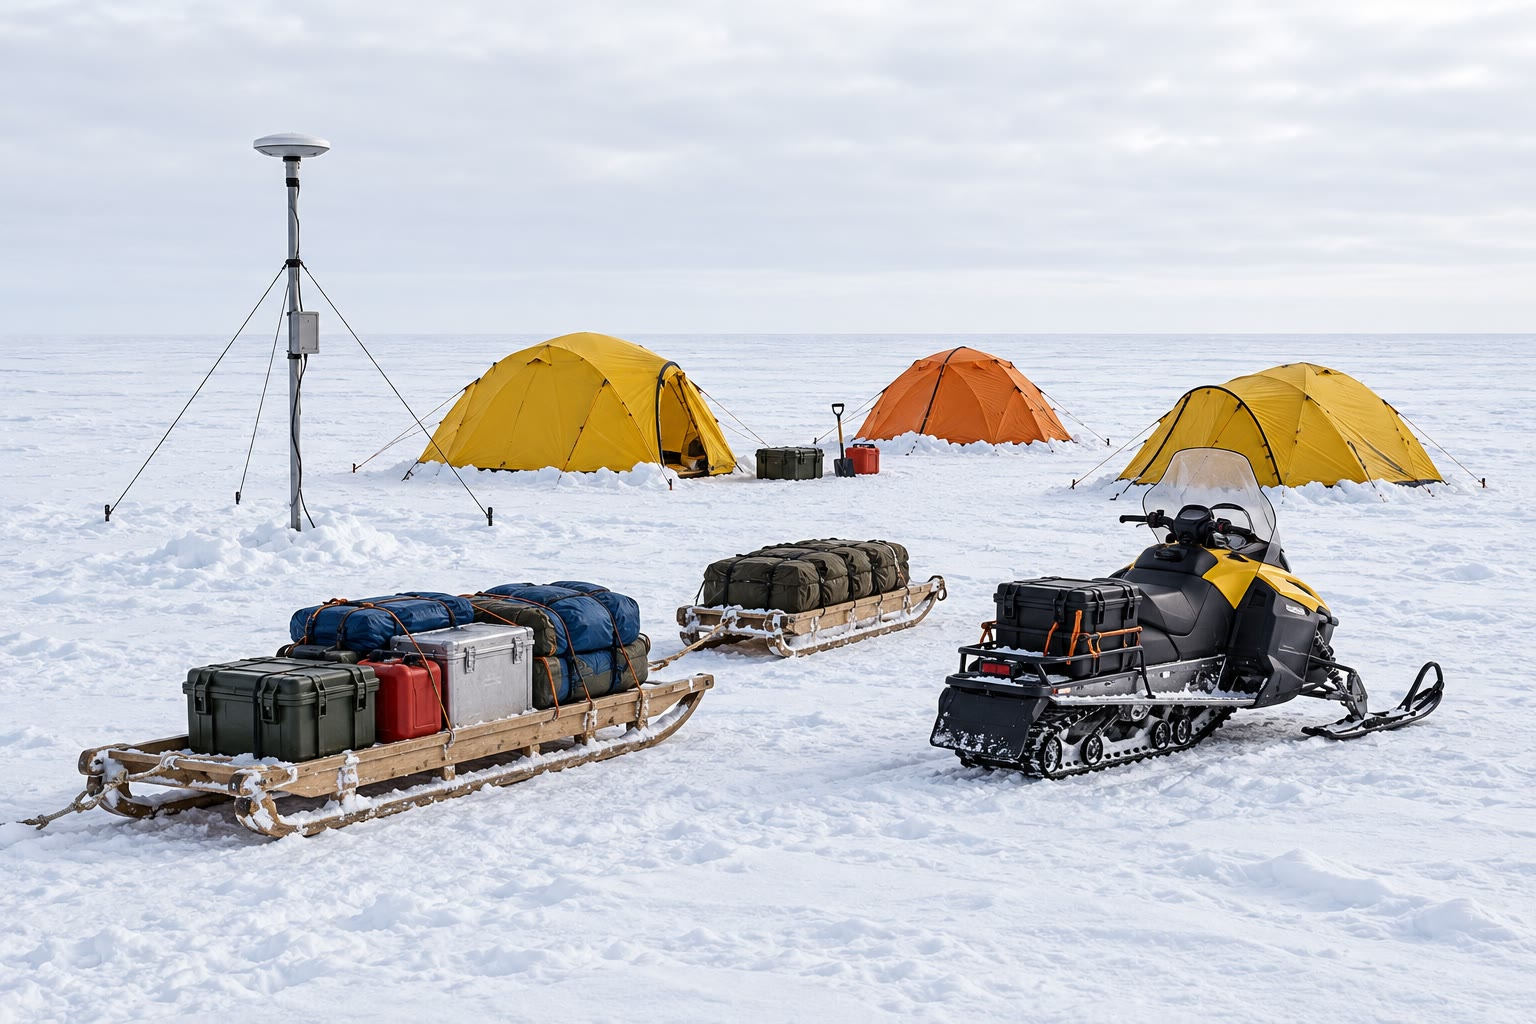
\includegraphics[width=\linewidth]{images/book5/ai/b3-glaciology-camp.jpg}

{\scriptsize مخيّم ميداني على غطاء جليدي: خيام، وزلّاجات،
ودراجة ثلج، وهوائي جهاز الملاحة بالأقمار الصناعية على سارية تشدّها
حبال الشدّ (رسم توضيحي مولَّد بالذكاء الاصطناعي).}
\end{minipage}
\end{inthefield}
% ledger: gps:high-end

\section{الجليد البحري والتربة الصقيعية}\label{sec:b3:glaciology:sea-ice}

يتشكّل الجليد البحري وينمو ويذوب في المحيط. وفي القطب الشمالي يبلغ
أكبر مساحة له في آذار وأصغرها في أيلول.
% ledger: nsidc:sea-ice-def

\begin{definition}[امتداد الجليد البحري]\label{def:b3:glaciology:sea-ice}
\emph{امتداد الجليد البحري}\index{امتداد الجليد البحري} هو المساحة الكلية
للخلايا في خريطة الأقمار الصناعية التي يغطّي فيها الجليد البحري أكثر من
\qty{15}{\percent} من السطح. وهو أكبر من مساحة الجليد البحري،
التي تحسب الجليد نفسه وحده.
\end{definition}
% ledger: nsidc:sea-ice-def

منذ أن بدأت الأقمار الصناعية رسم خرائطه عام 1979 تقلّص امتداد القطب الشمالي، في
آذار، وأكثر بكثير في أيلول: بمقدار \qty{0.74}{\mega km^2} لكل عقد في
أيلول، أي نحو \qty{12}{\percent} من متوسط الفترة 1981--2010 لكل عقد، مقابل
\qty{0.38}{\mega km^2}، و\qty{2.5}{\percent}، في آذار. وأصغر امتداد
لأيلول حتى الآن، \qty{3.57}{\mega km^2}، كان في عام 2012. يعكس
جليد البحر في القطب الشمالي \qtyrange{50}{70}{\percent} من ضوء الشمس، أمّا المحيط المفتوح
نحو \qty{6}{\percent}: فقدان الجليد يُعتِم السطح، وهذه هي التغذية الراجعة
بين الجليد والألبيدو، كما ورد في مجلد السنة الثانية.
% ledger: data:b5-nsidc-extent, nsidc:sea-ice-reflect

ينمو جليد البحر عند قاعدته، حيث يتجمّد عليه ماء البحر، والحرارة الكامنة
لهذا التجمّد يجب أن تنتقل بالتوصيل صعودًا عبر الجليد إلى الهواء البارد.

\begin{theorem}[قانون ستيفان]\label{thm:b3:glaciology:stefan}
جليد البحر ذو الموصلية الحرارية $k_i$، والكثافة $\rho_i$، والحرارة الكامنة للانصهار $L$،
إذا كان سطحه عند درجة حرارة أدنى بمقدار $\Delta T$ من نقطة
تجمّد الماء الذي تحته، فينمو إذا كانت الحرارة القادمة من المحيط
مهملة، وفق
\[
h(t)^2 - h(0)^2 = \frac{2k_i\,\Delta T}{\rho_iL}\,t .
\]
تحت طبقة من الثلج سماكتها $h_s$ وموصليتها $k_s$، يكون معدّل النموّ
هو $\mathrm dh/\mathrm dt = \Delta T/[\rho_iL(h/k_i + h_s/k_s)]$.
\end{theorem}

\begin{proof}
تكون درجة الحرارة في الجليد الرقيق خطّية، من نقطة التجمّد عند
القاعدة إلى درجة حرارة السطح عند الأعلى، لذا يكون الدفق الحراري عبره
$k_i\Delta T/h$، أو، عبر الجليد والثلج على التوالي، $\Delta T/(h/k_i +
h_s/k_s)$. يُطلق تجمّد طبقة $\mathrm dh$ حرارةً قدرها $\rho_iL\,\mathrm dh$ لكل
وحدة المساحة، ويجب أن يحمله هذا الدفق بعيدًا: $\rho_iL\,\mathrm dh/\mathrm dt
= k_i\Delta T/h$. ومنه $\mathrm d(h^2)/\mathrm dt = 2k_i\Delta T/(\rho_iL)$.
\end{proof}

بأخذ $k_i = \qty{2.03}{W.m^{-1}.K^{-1}}$، و$L = \qty{3.34e5}{J/kg}$،
و$\rho_i = \qty{917}{kg/m^3}$، فإنّ سطحًا أدنى بمقدار \qty{20}{K} من درجة التجمّد ينمو
\qty{1.5}{m} من الجليد خلال مائة يوم، و\qty{2.1}{m} خلال مائتي يوم.
أمّا الثلج، وموصليّته \qty{0.30}{W.m^{-1}.K^{-1}}، فهو عازل
جيّد: \qty{20}{cm} منه تُقلّص النموّ إلى أقلّ من النصف. ينمو الجليد السميك
ببطء والرقيق بسرعة: إذ يميل القانون إلى تسوية سماكة الجليد
بعد صيف من الذوبان.
% ledger: cice:constants, iapws:ice-density

\begin{omfigure}
\begin{tikzpicture}
\begin{groupplot}[group style={group size=2 by 1, horizontal sep=1.5cm},
  width=0.48\linewidth, height=0.4\linewidth,
  tick label style={font=\scriptsize}, label style={font=\small}, title style={font=\small}]
\nextgroupplot[xlabel={السنة}, ylabel={الامتداد \babelsublr{(\unit{\mega km^2})}}, xmin=1977, xmax=2028,
  ymin=0, ymax=18, title={امتداد الجليد البحري في القطب الشمالي},
  xticklabel style={/pgf/number format/1000 sep={}},
  legend style={font=\scriptsize, at={(0.03,0.66)}, anchor=west}]
% computed in figdata/bachelor-3/sea_ice.py
\addplot[omDef, thick, mark=*, mark size=0.9pt] table[x=year, y=mar] {figdata/out/bachelor-3-sea_ice-extent.dat};
\addlegendentry{مارس}
\addplot[omThm, thick, mark=*, mark size=0.9pt] table[x=year, y=sep] {figdata/out/bachelor-3-sea_ice-extent.dat};
\addlegendentry{سبتمبر}
\addplot[black!60, densely dashed, forget plot] table[x=year, y=mar] {figdata/out/bachelor-3-sea_ice-trend.dat};
\addplot[black!60, densely dashed, forget plot] table[x=year, y=sep] {figdata/out/bachelor-3-sea_ice-trend.dat};
\nextgroupplot[xlabel={أيام التجمّد}, ylabel={سماكة الجليد \babelsublr{(\unit{m})}}, xmin=0, xmax=200,
  ymin=0, ymax=2.4, title={النموّ، $\Delta T = \qty{20}{K}$},
  legend style={font=\scriptsize, at={(0.97,0.03)}, anchor=south east}]
\addplot[omMeth, thick] table[x=day, y=h0] {figdata/out/bachelor-3-sea_ice-stefan.dat};
\addlegendentry{جليد عارٍ}
\addplot[omDef, thick, densely dashed] table[x=day, y=hs] {figdata/out/bachelor-3-sea_ice-stefan.dat};
\addlegendentry{\foreignlanguage{arabic}{تحت طبقة ثلج بسماكة \mbox{\textdir TLT \qty{20}{cm}}}}
\end{groupplot}
\end{tikzpicture}

\par\smallskip{\small يسارًا، متوسط امتداد جليد البحر في القطب الشمالي في آذار وفي
أيلول للفترة 1979--2026 (الإصدار~4 من \babelsublr{NSIDC Sea Ice Index})، مع
اتجاهات المربعات الصغرى (بخط متقطّع): \qty{-0.38}{\mega km^2} و\qty{-0.74}{\mega km^2} لكل
عقد. يمينًا، نموّ جليد البحر بالتوصيل الحراري تحت سطح
\qty{20}{K} دون نقطة التجمّد، بلا حرارة من المحيط: الجليد العاري وفق قانون ستيفان،
والجليد نفسه تحت \qty{20}{cm} من الثلج.}\label{fig:b3:glaciology:sea-ice}
\end{omfigure}
% ledger: data:b5-nsidc-extent, cice:constants

التربة الصقيعية هي تربة تبقى عند \qty{0}{\celsius} أو دونها لمدة سنتين
أو أكثر. وهي تقع تحت نحو ربع اليابسة المكشوفة في نصف الكرة
الشمالي.
% ledger: nsidc:permafrost

\begin{definition}[الطبقة النشطة]\label{def:b3:glaciology:permafrost}
\emph{الطبقة النشطة}\index{الطبقة النشطة} هي الطبقة من التربة الواقعة فوق
التربة الصقيعية التي تذوب كل صيف وتتجمّد ثانيةً كل شتاء.
\end{definition}

يُحدَّد سمكها، كما في نموّ جليد البحر، بتوصيل الحرارة
إلى داخل التربة خلال موسم الذوبان، في مواجهة الحرارة الكامنة لجليد
التربة. وقد ارتفعت درجات حرارة التربة الصقيعية خلال ثلاثة إلى
أربعة عقود الماضية في جميع مناطق التربة الصقيعية (بدرجة ثقة عالية)؛
وارتفعت حرارة التربة الصقيعية عالميًّا بمقدار \qty{0.29}{\celsius} [\numrange{0.17}{0.41}]
بين 2007 و2016 (بدرجة ثقة متوسطة)، وأنّ زيادة سمك
\omterm{def:b3:glaciology:permafrost}{الطبقة النشطة} ظاهرة تشمل القطب الشمالي كلّه (بدرجة ثقة متوسطة).
وحيثما يذوب جليدها، قد تنهار التربة.
% ledger: ar6ch9:permafrost, nsidc:permafrost-thaw

\section{الغلاف الجليدي ومستوى سطح البحر}\label{sec:b3:glaciology:sea-level}

تضيف موازنة مستوى سطح البحر في مجلد السنة الثانية تمدّدَ المحيط الآخذ في الدفء
إلى الماء الذي يضيفه الجليد واليابسة. من
\qty{3.69}{mm/yr} المرصودة لارتفاع مستوى سطح البحر خلال 2006--2018، ساهمت الأنهار الجليدية
بمقدار \qty{0.62}{mm/yr}، وغرينلاند بمقدار \qty{0.63}{mm/yr}، وأنتاركتيكا
بمقدار \qty{0.37}{mm/yr}: فالجليد مجتمعًا يفوق تمدّد المحيط البالغ
\qty{1.39}{mm/yr}.
% ledger: ar6ch9:table95

\begin{dated}{2021}
غرينلاند فقدت \qty{4890}{Gt} من الجليد خلال 1992--2020 [4140 إلى 5640]،
\qty{13.5}{mm} من مستوى سطح البحر، بمعدّلات تصاعدت من \qty{39}{Gt/yr} في
التسعينيات إلى \qty{243}{Gt/yr} في 2010--2019، بالتصريف وبصورة متزايدة،
بالذوبان السطحي (بدرجة ثقة عالية). وفقدت أنتاركتيكا \qty{2670}{Gt}
[1800 إلى 3540]، \qty{7.4}{mm}، وتصاعد معدّلها من \qty{49}{Gt/yr} في
التسعينيات إلى \qty{148}{Gt/yr} في 2010--2019؛ وجاءت الخسائر من الأنهار الجليدية المصرّفة لغرب
أنتاركتيكا، أساسًا عن طريق ذوبان الرفوف الجليدية من الأسفل (بدرجة ثقة عالية).
وفقدت الأنهار الجليدية خارج الأغطية الجليدية \qty{6200}{Gt} خلال
1993--2019، \qty{17.1}{mm}، وكان الفقد أكبر في 2010--2019 منه في أيّ عقد آخر من
السجلّ (بدرجة ثقة عالية جدًّا). ستواصل غرينلاند فقدان الكتلة
طوال هذا القرن وفق جميع السيناريوهات المدروسة (شبه مؤكَّد)، وكذلك
أنتاركتيكا (مرجَّح): بحلول 2100 تضيف غرينلاند مرجَّحًا
\qtyrange{0.01}{0.10}{m} إلى مستوى سطح البحر تحت سيناريو منخفض الانبعاثات
و\qtyrange{0.09}{0.18}{m} تحت سيناريو مرتفع جدًّا، وأنتاركتيكا
\qtyrange{0.03}{0.27}{m} و\qtyrange{0.03}{0.34}{m}. من المرجَّح أن يصبح المحيط القطبي الشمالي
خاليًا عمليًّا من جليد البحر، بأقلّ من
\qty{1}{\mega km^2} منه، عند حدّه الأدنى في أيلول لأوّل مرّة
قبل 2050 وفق جميع السيناريوهات المدروسة.
\end{dated}
% ledger: ar6ch9:greenland, ar6ch9:antarctica, ar6ch9:glaciers, ar6ch9:ice-sheet-proj, ar6ch9:sea-ice

خسائر الغطاء الجليدي هي تلك الواردة في الفصل~\ref{ch:b3:gravity-geodesy}،
تُقاس بقياس الارتفاع، وبقياس الجاذبية، وبالفرق بين الثلج
الذي يتساقط والجليد الذي يتدفّق خارجًا: ثلاث طرق مستقلّة جُمعت
في تقدير واحد.
% ledger: data:b5-imbie

\section{التمارين}

\begin{exercise}[$\star$]\label{exo:b3:glaciology:1}
نهرٌ جليدي وادٍ سماكته \qty{250}{m} يتدفّق على منحدر \ang{3}. احسب
إجهاد القصّ عند القاعدة، وقارنه بإجهادات القاعدة في الأنهار الجليدية الحقيقية،
وهي من مرتبة بار واحد.
\end{exercise}

\begin{exercise}[$\star$]\label{exo:b3:glaciology:2}
(أ)~يحتوي الغطاء الجليدي في غرينلاند على نحو \qty{2.9}{\mega km^3} من الجليد،
كثافته \qty{917}{kg/m^3}. احسب كتلته ومكافئها من مستوى سطح البحر عند
\qty{360}{Gt/mm}، وقارنه بالقيمة \qty{7.4}{m} التي تُذكر عادةً.
(ب)~افعل الشيء نفسه لأنتاركتيكا \qty{30}{\mega km^3}، المذكورة بقيمة نحو
\qty{58}{m}. لماذا تختلف نتيجتا المقارنة إلى هذا الحد؟
\end{exercise}
% ledger: nsidc:ice-sheets

\begin{exercise}[$\star$]\label{exo:b3:glaciology:3}
لنهر جليدي نطاق تراكم مساحته \qty{6}{km^2} وميزان متوسط قدره
\qty{+1.2}{m} مكافئ ماء، ونطاق استنزاف مساحته \qty{4}{km^2} وميزانه
\qty{-2.1}{m}. احسب صافي الميزان بالأمتار المكعبة من الماء، ومتوسط
الميزان النوعي، ونسبة مساحة \omterm{def:b3:glaciology:mass-balance}{نطاق التراكم}. هل هو في تزايد أم
في تناقص؟
\end{exercise}

\begin{exercise}[$\star$]\label{exo:b3:glaciology:4}
عند \omterm{def:b3:glaciology:firn}{انغلاق المسام} تبلغ كثافة \omterm{def:b3:glaciology:firn}{الفِرن} \qtyrange{820}{830}{kg/m^3}.
ما كسر حجمه الذي ما يزال فراغًا مساميًّا (كثافة الجليد:
\qty{917}{kg/m^3})؟
\end{exercise}
% ledger: firn:close-off

\begin{exercise}[$\star\star$]\label{exo:b3:glaciology:5}
نهرٌ جليدي معتدل (الجليد عند \qty{0}{\celsius}، $A =
\qty{1.4e-16}{Pa^{-3}.yr^{-1}}$) سماكته \qty{300}{m} على منحدر
\ang{3}. احسب سرعة السطح بالتشوّه الداخلي وحده. بأيّ عامل
تتغيّر السرعة لو كان سمكه ضعف ما هو عليه؟ وماذا لو كان المنحدر
نصف قيمته؟
\end{exercise}

\begin{exercise}[$\star\star$]\label{exo:b3:glaciology:6}
انطلاقًا من ثوابت باترسون--بود، احسب \omterm{def:b3:glaciology:glen}{عامل المعدّل} عند
\qty{-25}{\celsius} و\qty{-10}{\celsius}، ونسبة سرعتي
كتلتين جليديتين متماثلتين عند \qty{0}{\celsius} وعند \qty{-25}{\celsius}.
\end{exercise}
% ledger: pism:rheology, codata:R

\begin{exercise}[$\star\star$]\label{exo:b3:glaciology:7}
احسب أكبر سماكة لغطاء جليدي لدن يمتدّ \qty{1000}{km} من
المركز إلى الحافة، مع $\tau_0 = \qty{100}{kPa}$، وقارنها بأكبر
سماكة للجليد الأنتاركتيكي، نحو \qty{4.9}{km}.
\end{exercise}
% ledger: nsidc:ice-sheets

\begin{exercise}[$\star\star$]\label{exo:b3:glaciology:8}
نهرٌ جليدي سماكته \qty{200}{m} يفقد \qty{5}{m} من الجليد سنويًّا عند لسانه.
قدّر زمن استجابته. لو ارتفعت حرارة المناخ فجأةً ثم استقرّت
ثابتة، فكم من الزمن سيستمرّ طوله في التغيّر؟
\end{exercise}

\begin{exercise}[$\star\star$]\label{exo:b3:glaciology:9}
(أ)~باستخدام قانون ستيفان مع $\Delta T = \qty{20}{K}$، احسب سماكة
الجليد البحري العاري بعد 100 يومًا، والزمن اللازم لبلوغ \qty{3}{m}.
(ب)~ماذا يوحي ذلك بشأن الجليد الأسمك من \qty{3}{m}؟
\end{exercise}
% ledger: cice:constants

\begin{exercise}[$\star\star\star$]\label{exo:b3:glaciology:10}
(أ)~حيث يقع القاع على عمق \qty{800}{m} تحت مستوى سطح البحر، كم سماكة الجليد عند
\omterm{def:b3:glaciology:grounding-line}{خط الارتكاز}؟ (ب)~باستخدام دفق اللوح المندس $q \propto H^{n+2}$ عند منحدر سطحي معيّن،
بأيّ عامل يزداد دفق الجليد المرتكز إذا تراجع
\omterm{def:b3:glaciology:grounding-line}{خط الارتكاز} حتى يصبح القاع على عمق \qty{900}{m}؟ (ج)~فسّر
لماذا يجعل تعمّق القاع نحو الداخل التراجعَ ذاتيَّ التعزيز، وما الذي
يغيّره الرفّ الجليدي.
\end{exercise}
% ledger: iapws:ice-density, noaa:seawater-1025

\begin{exercise}[$\star\star\star$]\label{exo:b3:glaciology:11}
أثبت أنّ حجم قبّة جليدية لدنة دائرية نصف قطرها $R$ هو $V =
\frac{8\pi}{15}\sqrt{2\tau_0/(\rho g)}\,R^{5/2}$. بأيّ عامل يزداد
مكافئها من مستوى سطح البحر إذا تضاعف نصف قطرها؟
\end{exercise}

\begin{exercise}[$\star\star\star$]\label{exo:b3:glaciology:12}
بلغ متوسط \omterm{def:b3:glaciology:sea-ice}{امتداد الجليد البحري} في القطب الشمالي \qty{16.34}{\mega km^2} في آذار 1979،
و\qty{14.13}{\mega km^2} في آذار 2026، وفي أيلول \num{7.05}
و\qty{4.81}{\mega km^2}. (أ)~احسب التغيّر النسبي في كلّ شهر.
(ب)~أعطِ سببين فيزيائيين يفسّران لماذا تراجع امتداد أيلول إلى هذا الحدّ
أسرع من امتداد آذار بكثير.
\end{exercise}
% ledger: data:b5-nsidc-extent

\section{مسألة: قبّة أركيل الجليدية}

\begin{problem}[{مسألة نهاية الأسبوع --- شكل القبّة الجليدية وانسيابها وميزانها
ومكافئها من مستوى سطح البحر لقبّة جليدية افتراضية}]
\label{pb:b3:glaciology:1}
تقع قبّة أركيل الجليدية الافتراضية على هضبة مستوية. وهي شبه دائرية
\qty{20}{km} نصف قطرها، ودرجة حرارة جليدها نحو \qty{-10}{\celsius}. خذ
$\rho = \qty{917}{kg/m^3}$ و$g = \qty{9.81}{m/s^2}$.

\medskip\noindent\textbf{الجزء الأول --- هل القبّة لدنة؟}
\begin{enumerate}
\item أثبت أنّ إجهاد القصّ القاعدي تحت جليد سماكته $H$ وبمنحدر سطحي صغير
  $\alpha$ يساوي تقريبًا $\rho gH\alpha$.
\item تُعطي القياسات الرادارية والمسوح على بعد 5 و10 و\qty{15}{km} من المركز
  سماكات قدرها 580 و470 و\qty{335}{m}، ومنحدرات سطحية قدرها
  \num{0.0190}، \num{0.0240} و\num{0.0330}. احسب إجهاد القصّ القاعدي
  عند النقاط الثلاث.
\item هل القبّة قريبة من اللدونة؟ وما إجهاد الخضوع الذي يُعتمد؟
\item مع $\tau_0 = \qty{100}{kPa}$، احسب $2\tau_0/(\rho g)$.
\item توقّع السماكة عند النقاط الثلاث انطلاقًا من المقطع اللدن
  وقارنها بالقياسات الرادارية.
\end{enumerate}

\medskip\noindent\textbf{الجزء الثاني --- الشكل والحجم.}
\begin{enumerate}[resume]
\item احسب السماكة عند المركز.
\item أثبت أنّ الحجم هو $V = \frac{8\pi}{15}\sqrt{2\tau_0/(\rho
  g)}\,R^{5/2}$.
\item احسب الحجم بالكيلومترات المكعّبة.
\item احسب المساحة والسماكة المتوسطة.
\item قبّة جليدية أوسع مرّتين على الهضبة نفسها: بأيّ عامل
  يكون حجمها أكبر؟
\end{enumerate}

\medskip\noindent\textbf{الجزء الثالث --- التدفّق والميزان.}
\begin{enumerate}[resume]
\item احسب \omterm{def:b3:glaciology:glen}{عامل المعدّل} عند \qty{-10}{\celsius} في
  \unit{Pa^{-3}.yr^{-1}}.
\item عند \qty{10}{km} من المركز، معتبرًا الجليد لوحًا، احسب
  سرعة السطح الناتجة عن التشوّه الداخلي.
\item احسب تدفّق الجليد لكلّ وحدة عرض هناك، ومتوسط سرعة
  العمود.
\item في الحالة المستقرّة، يساوي التدفّق الخارج من الدائرة التي نصف قطرها
  \qty{10}{km} الميزانَ المكتسب داخلها. ما متوسط الميزان
  الذي يتطلّبه ذلك، بالأمتار من الجليد في السنة؟
\item يقع خطّ التوازن على ارتفاع \qty{450}{m} فوق الهضبة. أين يقع
  على القبّة، وما نسبة مساحة \omterm{def:b3:glaciology:mass-balance}{نطاق التراكم}؟
\item إذا ارتفعت حرارة الجليد إلى \qty{0}{\celsius}، بأيّ عامل ستزداد
  السرعات؟ وماذا سيحدث لشكل القبّة؟
\end{enumerate}

\medskip\noindent\textbf{الجزء الرابع --- مستوى سطح البحر.}
\begin{enumerate}[resume]
\item احسب كتلة القبّة بالغيغاطن.
\item احسب \omterm{def:b3:glaciology:sle}{مكافئ مستوى سطح البحر} لها بالميليمترات.
\item إذا رقّت القبّة كلّها بمقدار \qty{0.5}{m} من الجليد في السنة، دون
  أن تتدفّق، فكم ستدوم؟
\item لماذا ستزول القبّة الحقيقية قبل ذلك، بمجرّد أن تبدأ
  بالترقّق؟
\item بالمعدّل الذي فقدت به غرينلاند الجليد في 2010--2019، كم سيستغرق
  فقدان كتلة تعادل قبّة أركل؟
\item أعطِ \omterm{def:b3:glaciology:sle}{مكافئ مستوى سطح البحر} لقبّة أركل الجليدية بالميليمترات،
  مقرّبًا إلى منزلة عشرية واحدة.
\end{enumerate}
\end{problem}
% ledger: pism:rheology, data:b5-imbie, ar6ch9:greenland, ar6ch9:faq91
